\chapter{Opis projektnog zadatka}
		
		
		\textit U okviru projekta za razvoj programske potpore cilj nam je napraviti web aplikaciju 
“Pomozi mi“ čiji je primarni zadatak mogućnost traženja pomoći te pružanje same usluge od strane ljudi koji žele pomagati. Potencijalna korist mogla bi biti i samo zbližavanje korisnika te širenje osjećaja sigurnosti i povezanosti same zajednice. Na ovaj način mnogi ljudi kojima je odlazak u trgovinu ili košnja trave veliki izazov pronalaze način da dođu do osoba koji svoj višak vremena žele iskoristiti za pomaganje potrebitijima. Iako danas postoje mnoge društvene mreže, ova stranica nema nepotreban sadržaj te je maksimalno prilagođena svojoj funkciji uz jednostavno korištenje. \newline
Prvi korak prema korištenju usluga same aplikacije je prijava u sustav.
Svaki korisnik aplikacije ukoliko nema otvoreni profil (javni korisnik) se mora registrirati. Prilikom registracije ostavlja osnovne podatke o sebi :

		\begin{packed_item}
			\item \textit Ime
			\item \textit Prezime
			\item \textit Lozinka
			\item \textit Adresa
			\item \textit e-mail
		\end{packed_item}
		
		\textit Za svako sljedeće korištenje dovoljna je prijava pomoću e-mail adrese i lozinke.

Nakon prijave korisnik može pristupiti pregledu svog profila, listi korisnika ili odabrati neku od dvije aktivnosti same aplikacije: nudi li pomoć ili je traži te s obzirom na odabir se otvara odgovarajuća stranica. 

		\eject

		%unos slike
		\begin{figure}[H]
			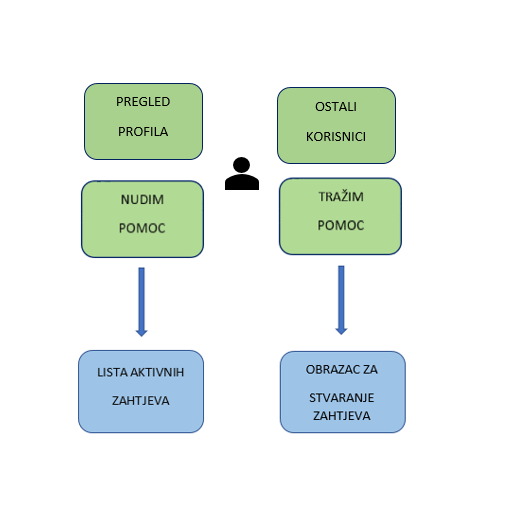
\includegraphics[scale=0.6]{slike/projekt1.png} %veličina slike u odnosu na originalnu datoteku i pozicija slike
			\centering
			\caption {odabir nakon prijave}
			\label{fig:promjene}
		\end{figure}
		
		\textit Kada korisnik traži pomoć ispunjava obrazac za stvaranje zahtijeva. Na njemu unosi sljedeće podatke:
		
		\begin{packed_item}
			\item \textit Kratki opis posla
			\item \textit Kontakt: broj mobitela / e-mail
			\item \textit Opcionalno datum i vrijeme
			\item \textit Opcionalno lokacija
		\end{packed_item}

        \textit Ukoliko je lokacija važna za izvršavanje usluge može se dohvatiti s uređaja ili označiti na karti.
        \newline
Nakon objave korisnik je autor zahtjeva te je u mogućnosti zahtjev obrisati trajno iz baze podataka ili ga trenutno blokirati. Objavljeni zahtjev se nalazi na listi aktivnih zahtjeva.
\newline
Svi koji žele pomoći, na stranici aktivnih zahtjeva pronalaze koju uslugu bi mogli izvršiti. Prilikom pregleda liste moguće je lako dohvatiti profil korisnika koji je objavio zahtjev.Svakom korisniku se prikazuju samo zahtjevi čija je lokacija unutar jednog kilometra od uređaja korisnika te zahtjevi za čije je izvršavanje lokacija nebitna. Kada korisnik pronađe zadovoljavajuću ponudu usluge odabire izvršavanje čime postaje izvršitelj zahtjeva.

        		%unos slike
		\begin{figure}[H]
			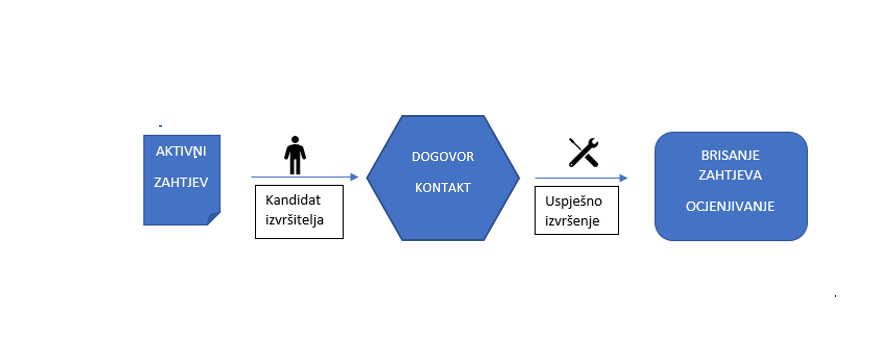
\includegraphics[scale=0.7]{slike/projekt2.png} %veličina slike u odnosu na originalnu datoteku i pozicija slike
			\centering
			\caption {proces izvršavanja zahtjeva}
			\label{fig:promjene}
		\end{figure}

        \textit Odabirom posla šalje se automatska obavijest autoru zahtjeva o potencijalnom izvršitelju. Izvršitelj i autor mogu dodatno pojasniti sam posao i ostale detalje izvedbe. Nakon što je usluga obavljena autor zahtjev označava kao izvršen te se briše s liste aktivnih.  
        \newline
Nakon izvršenja posla moguće je ocijeniti drugog korisnika ocjenama 1-5 te ostaviti komentar. Ocjenjivanje je moguće i kad si korisnici nisu međusobno pomagali, a sve ocjene i komentari su vidljivi na profilu korisnika.
        \newline
Svaki korisnik svoj profil može vidjeti u svakom trenutku, a ostale korisnike može pretražiti ili ih dohvatiti među aktivnim zahtjevi. Na tuđim profilima su vidljivi :
		
		\begin{packed_item}
			\item \textit Ime
			\item \textit Prezime
			\item \textit Ocjena korisnika
			\item \textit "lanac povjerenja"

		\end{packed_item}
		
		
“Lanac povjerenja“ prikazuje kako su ljudi koje sami ocijenimo visoko ocijenili profil koji trenutno gledamo. Na taj način korisnik se sigurnije osjeća za daljnju komunikaciju s korisnikom profila.
\newline
Kada korisnik gleda vlastiti profil ima mogućnost pristupa listi vlastitih zahtjeva. Unutar liste vlastitih zahtjeva bira pregled izvršenih ili aktivnih kojima može dodatno upravljati. Zahtjevi su sortirani vremenski, a moguće su još dodatne opcije filtriranja poput kategorije i lokacije. Svi zahtjevi koji su aktivni, izvršeni ili blokirani ostaju pohranjeni u bazi podataka.
\newline

Osim korisnika važnu ulogu imaju administratori koji su dodijeljeni za određenu geografsku lokaciju. Oni brinu da sadržaj koji se objavljuje ne bude lažan ili opasan te imaju mogućnost brisanja zahtjeva i profila. Oni mogu privremeno ili trajno blokirati sve korisnike aplikacije.
\newline
Ova aplikacija se lako po potrebi može proširiti i na druga područja uz male preinake vrsta zahtjeva. Također ukoliko se uoči potreba moguće je lako stvoriti i mobilnu aplikaciju koja bi još dodatno olakšala sam pristup korisnicima.

\eject
		
	